\section{Simulation Analysis}
\label{sec:simulation}


\subsection{Operating Point Analysis for t\textless0}

Table~\ref{tab:op1} shows the simulated operating point results for the circuit
under analysis. Compared to the theoretical analysis results, we can see that the values are exactly the same.

\begin{table}[ht]
  \centering
  \begin{tabular}{|l|r|}
    \hline    
    {\bf Name} & {\bf Value [A or V]} \\ \hline
    \input{values1_tab}
  \end{tabular}
  \caption{Operating point. A variable preceded by @ is of type {\em current}
    and expressed in Ampere; other variables are of type {\it voltage} and expressed in
    Volt.}
  \label{tab:op1}
\end{table}



\subsection{Operating Point Analysis for vs(t)=0}

Table~\ref{tab:op2} shows the simulated operating point results for the circuit, this time with the null voltage source and with the replacement of the capacitor by a voltage source $V_x=V(6)-V(8)$. This procedure is necessary to determine the initial conditions, in this case they correspond to the ones of a saturated capacitor. 

\begin{table}[ht]
  \centering
  \begin{tabular}{|l|r|}
    \hline    
    {\bf Name} & {\bf Value [A or V]} \\ \hline
    \input{values2_tab}
  \end{tabular}
  \caption{Operating point. A variable preceded by @ is of type {\em current}
    and expressed in Ampere; other variables are of type {\it voltage} and expressed in
    Volt.}
  \label{tab:op2}
\end{table}

\newpage

\subsection{Simulation of the natural response of the circuit}

In this point we have simulated the natural response of the circuit, using the boundary conditions V(6) and V(8) as obtained in 3.2). Then we used Ngspice’s transient analysis mode to get v6(t) in the interval [0, 20] ms. Finally we have plotted the result, as you can see in Figure 10. This plot is equal to the one get in the theoretical analyses
\vspace{-0.9in}
\begin{figure}[H] \centering
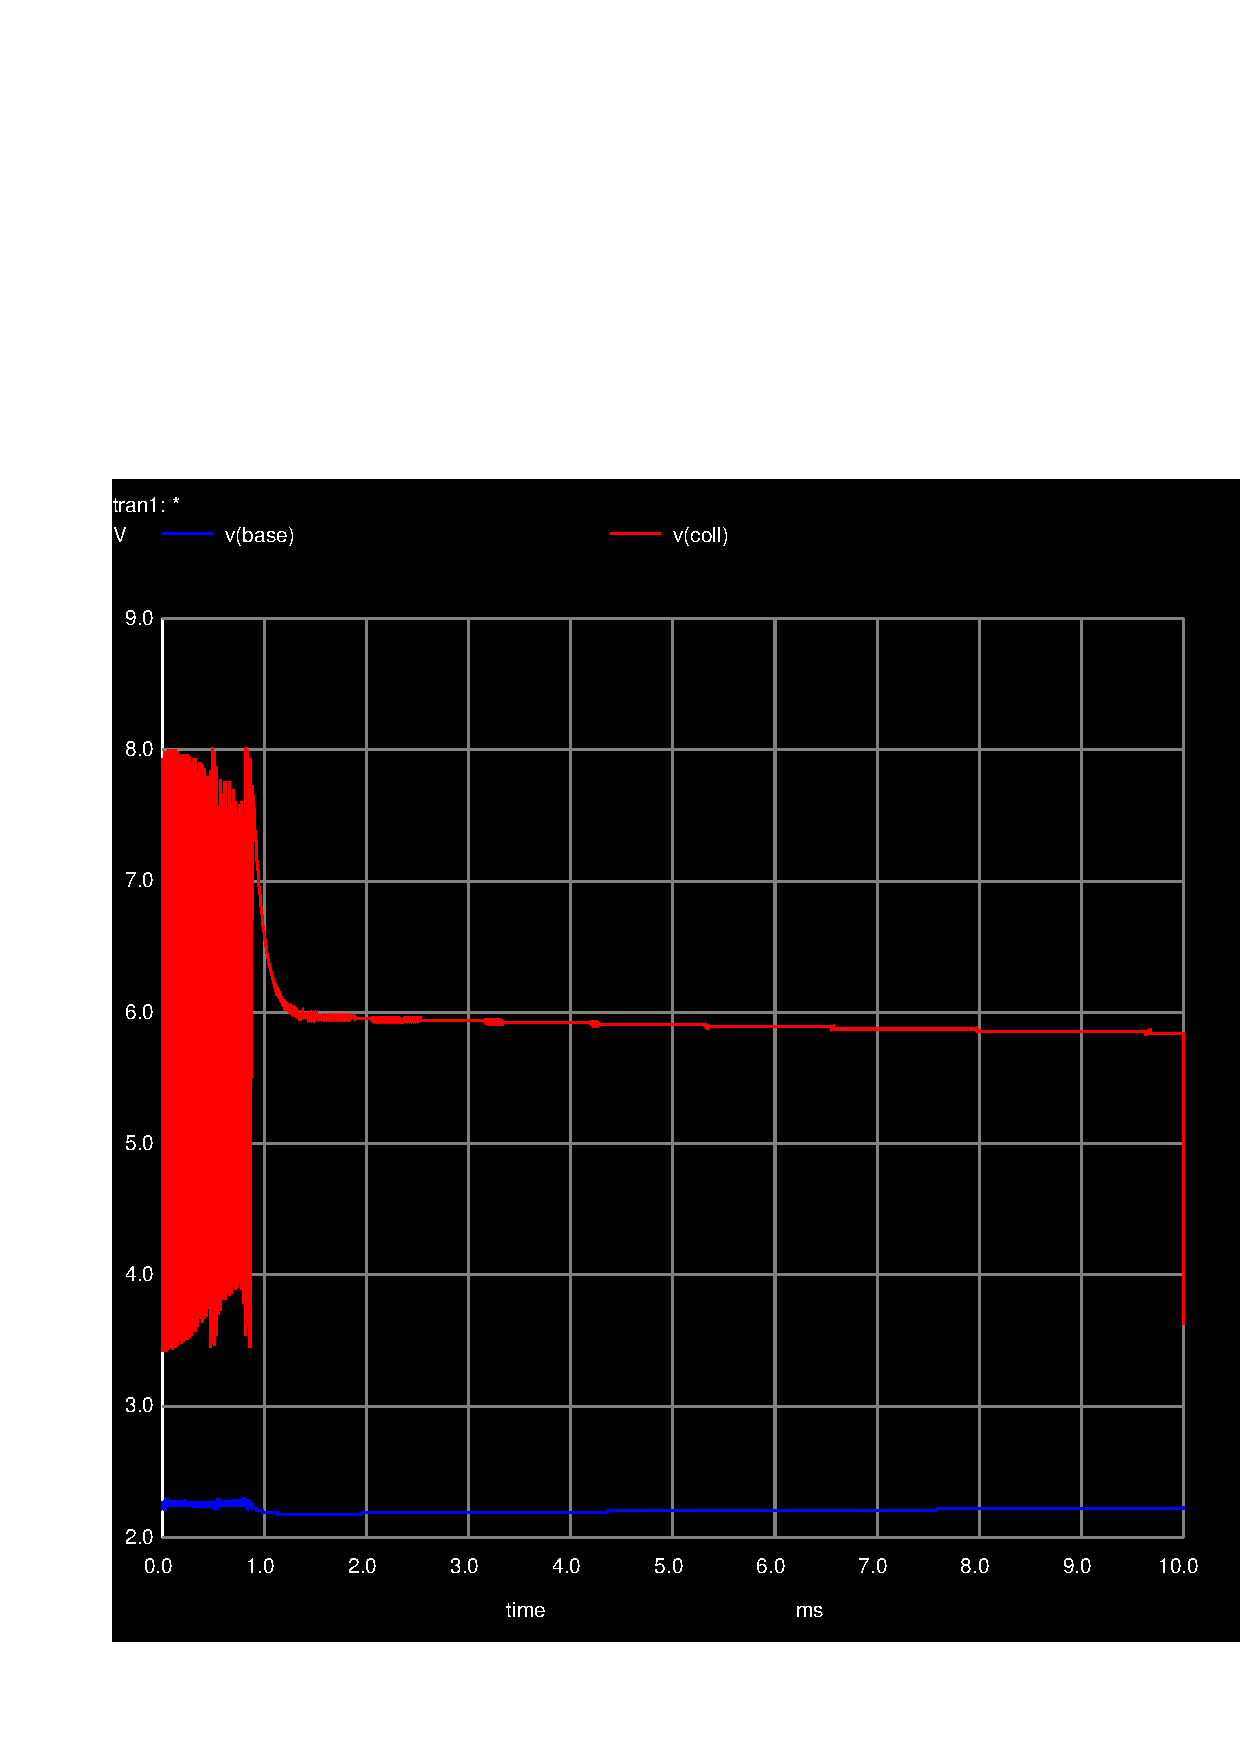
\includegraphics[width=0.45\linewidth]{trans.pdf}
\caption{Transient natural response output of voltage V6}
\label{fig:trans}
\end{figure}



\subsection{Simulation of the natural and forced response of the circuit}


We simulated the natural and forced response on node 6 by repeating step  3) (3.3) with $v_s(t)$ as given in Fig. 1 and with f=1kHz. Then we plotted both the stimulus and the response.
\vspace{-1.2in}
\begin{figure}[H] \centering
\includegraphics[width=0.45\linewidth]{trans2.pdf}
\caption{Transient total response output voltage V6}
\label{fig:trans2}
\end{figure}



\subsection{Simulation of the frequency response in node 6 } 

The next point was to do the response in frequency, as it was already referred, the increase in frequency, decreases the capacitor impedance, this is, the tension will decrease. This is the reason why we observe a negative variation in terms of magnitude in the Bode's diagram, since 10Hz to $10^4$ Hz. With the influence of this frequency the variation on the capacitor is so small, that is not going to interfere with v6. As Vs is a voltage source both its magnitude and phase do not change.

\vspace{-0.9in}

\begin{figure}[H] \centering
\includegraphics[width=0.45\linewidth]{acmag.pdf}
\caption{Frequency response (Bode Diagram: Magnitude)}
\label{fig:acmag}
\end{figure}

\vspace{-1in}

\begin{figure}[H] \centering
\includegraphics[width=0.45\linewidth]{acphase.pdf}
\caption{Frequency response (Bode Diagram: Phase)}
\label{fig:acphase}
\end{figure}

\newpage


